\section{Implicit condensation and expansion}\label{sec:vf-ice}

\subsection*{Concept and purpose}

\citet{hollkamp2008ice} reduce a geometrically nonlinear beam to a few bending modes and identify the nonlinear modal force from static solutions of the full-order model (implicit condensation). Because the linear bending modes of a straight beam have no axial component, the reduced model predicts no in-plane displacement, and the paper recovers it by a second step, the expansion: the in-plane displacement is regressed on the quadratic products of the modal amplitudes. The reduced model is then driven by a random load and compared with the full-order response in time and in the power spectrum, and its in-plane response and stress are recovered. The study tests the identification, the dynamic prediction at two excitation levels, the in-plane expansion and the stress recovery, and the training strategy behind them.

The study uses \anchor{fea_engine.elements.Beam2DCorotational}, the static-fit and polynomial ROM classes of \rom{}, the reduced Newton--Newmark integrator \anchor{rom_engine.integrate_newmark_surrogate} (promoted from the study's prototype) and \anchor{rom_engine.membrane_expansion} for the one-mode expansion. The package gaps found while reproducing (membrane expansion, a multi-mode training strategy, a robust reduced Newton integrator, fibre stress recovery, a band-limited load generator) are recorded in the study's gap analysis, and three of them were closed in the process.

\subsection*{Mathematics as implemented}

With $n$ mass-normalised bending modes, $\boldsymbol\Phi_b^{T}\mathbf M\boldsymbol\Phi_b=\mathbf I$ and $\boldsymbol\Phi_b^{T}\mathbf K\boldsymbol\Phi_b=\boldsymbol\Lambda=\operatorname{diag}(\omega_i^2)$, and $\mathbf u\approx\boldsymbol\Phi_b\mathbf p$, the full-order model $\mathbf M\ddot{\mathbf u}+\mathbf C\dot{\mathbf u}+\mathbf K\mathbf u+\mathbf f_{\rm nl}(\mathbf u)=\mathbf F(t)$ reduces to
\begin{equation}\label{eq:ice-rom}
\ddot p_i+\sum_j\bar c_{ij}\dot p_j+\omega_i^2p_i+\theta_i(\mathbf p)=f_i(t),\qquad\mathbf f=\boldsymbol\Phi_b^{T}\mathbf F,\quad\bar c_{ij}=(\boldsymbol\Phi_b^{T}\mathbf C\boldsymbol\Phi_b)_{ij},
\end{equation}
with the nonlinear modal force in the quadratic-plus-cubic form
\begin{equation}\label{eq:ice-theta}
\theta_i(\mathbf p)=\sum_{j\le k}B_i(j,k)\,p_jp_k+\sum_{j\le k\le l}A_i(j,k,l)\,p_jp_kp_l .
\end{equation}
For a flat structure symmetry removes the quadratic terms and every cubic term with three distinct modes (paper Eq.~7),
\begin{equation}\label{eq:ice-restr}
B_i(j,k)=0,\qquad A_i(j,k,l)=0\ \text{ if $j,k,l$ pairwise distinct},
\end{equation}
which for $n=4$ leaves four self-cubic terms $p_i^3$ and twelve two-mode terms $p_i^2p_j$, 16 coefficients per equation as in the paper; the unrestricted form has 30 (10 quadratic, 20 cubic), and one mode keeps $A_1p_1^3$ only.

\emph{Identification.} Each static sample applies $\mathbf F_s=\mathbf M\boldsymbol\Phi_b\hat{\mathbf f}_s$ and solves the nonlinear static problem for $\mathbf u_s$; projection gives
\begin{equation}\label{eq:ice-id}
\mathbf p_s=\boldsymbol\Phi_b^{T}\mathbf M\mathbf u_s,\qquad\boldsymbol\theta_s=\hat{\mathbf f}_s-\boldsymbol\Lambda\mathbf p_s,
\end{equation}
and the coefficients solve a linear least-squares problem with the monomials of \cref{eq:ice-theta,eq:ice-restr} as the columns of $\boldsymbol\Pi$,
\begin{equation}\label{eq:ice-ls}
\mathbf c=\arg\min_{\mathbf c}\lVert\boldsymbol\Theta-\mathbf c\,\boldsymbol\Pi\rVert_F^2=\boldsymbol\Theta\,\boldsymbol\Pi^{+}.
\end{equation}

\emph{Membrane expansion.} With snapshots $\mathbf W=[\mathbf u_1\cdots\mathbf u_S]$, amplitudes $\mathbf P$ and the quadratic monomials $\mathbf q=[p_1^2,\,p_1p_2,\,\dots,\,p_n^2]^{T}$,
\begin{equation}\label{eq:ice-exp}
\mathbf W-\boldsymbol\Phi_b\mathbf P\approx\mathbf T_m\mathbf Q,\quad\mathbf T_m=[\mathbf W-\boldsymbol\Phi_b\mathbf P]\mathbf Q^{+},\quad\mathbf u(t)=\boldsymbol\Phi_b\mathbf p(t)+\mathbf T_m\mathbf q(t).
\end{equation}
Only the one-mode case is implemented, where $\mathbf q=p_1^2$ and $\mathbf T_m=\sum_s(\mathbf u_s-\boldsymbol\phi_1p_{1,s})\,p_{1,s}^2\big/\sum_sp_{1,s}^4$.

\emph{Reduced Newton--Newmark.} At each step the residual and Jacobian
\begin{equation}\label{eq:ice-newton}
\mathbf R(\mathbf p_{n+1})=\ddot{\mathbf p}_{n+1}+\bar{\mathbf C}\dot{\mathbf p}_{n+1}+\boldsymbol\Lambda\mathbf p_{n+1}+\boldsymbol\theta(\mathbf p_{n+1})-\mathbf f_{n+1},\qquad
\mathbf J=\frac{\mathbf I}{\beta\Delta t^2}+\frac{\gamma\bar{\mathbf C}}{\beta\Delta t}+\boldsymbol\Lambda+\frac{\partial\boldsymbol\theta}{\partial\mathbf p}
\end{equation}
are formed with $\ddot{\mathbf p}_{n+1}$ and $\dot{\mathbf p}_{n+1}$ written through $\mathbf p_{n+1}$ by the Newmark relations, with a line search and an amplitude clamp.

\emph{Fibre stress.} The axial stress at fibre height $y$ of an element is
\begin{equation}\label{eq:ice-stress}
\sigma(\xi,y)=E\left(\frac{\bar e}{L_0}-y\,\kappa(\xi)\right),
\end{equation}
with $\bar e$ the corotational axial extension, $L_0$ the reference length and $\kappa$ the curvature from the corotational end rotations.

\emph{Metric.} All dynamic errors are $\varepsilon=\operatorname{rms}(v_{\rm ROM}-v_{\rm FOM})/\operatorname{rms}(v_{\rm FOM})$ for the transverse displacement at $x=4$~in; a value above 1 means the ROM error exceeds the signal.

\subsection*{Geometry and mesh}

The structure is the aluminium beam of the publication, $18\times1\times0.09$~in, clamped at both ends with immovable ends (\Cref{fig:vf-ice-geom}). The publication models the symmetric half with 36 elements; here the full beam is meshed with 36 \texttt{Beam2DCorotational} elements ($\Delta x=0.5$ in) and the symmetric modes are picked by a mirror-symmetry score above $0.9$. \Cref{tab:vf-ice-setup} lists what is shared with the publication and what was chosen.

\begin{figure}[tbp]
\centering
\includegraphics[width=0.98\linewidth]{figures/ch14_geom_ice.pdf}
\caption{Flat beam of the ICE study, drawn from the dimensions of the report: 36 elements, clamped ends, the observation point at $x=4$ in and the spatially uniform random load.}\label{fig:vf-ice-geom}
\end{figure}

\begin{table}[tbp]
\centering\footnotesize
\caption{Set-up of the ICE study.}\label{tab:vf-ice-setup}
\begin{tabularx}{\linewidth}{@{}>{\raggedright\arraybackslash}p{2.8cm} >{\raggedright\arraybackslash}X >{\raggedright\arraybackslash}X@{}}
\toprule
Item & Publication & This work\\
\midrule
Geometry, material & $18\times1\times0.09$ in; $E=10.6\times10^6$ psi, $G=4.0\times10^6$ psi, $\rho=2.588\times10^{-4}$ lb s$^2$/in$^4$ & same ($\nu=0.325$)\\
Mesh & symmetric half, 36 elements & full beam, 36 elements\\
Retained modes & 4 symmetric bending modes & 1 and 4\\
Excitation & uniform, Gaussian, band-limited 0--1500 Hz, 0.9216 and 0.0072 lb/in RMS & same; spectral synthesis, seed 42\\
Damping & not recorded here & Rayleigh, mass-proportional, $\zeta_1=0.02$, in FOM and ROM\\
Time integration & not recorded here & 20\,000 steps, $\Delta t=5\times10^{-5}$ s, $T=1$ s; implicit Newmark (FOM about 240 s per run)\\
Training, 4 modes & not stated & 150 static solves, target $\pm3\times0.09$ in per mode (Latin hypercube), 12 held out\\
Training, 1 mode & not stated & 60 samples at $\pm150$, 15 held out (set A); 20 samples at $\pm3$ (set B)\\
Neural surrogate & none & multilayer perceptron (MLP), 4000 epochs, 150 static samples\\
Trajectory states & none & 80 states from short FOM transients (6\,002 visited) added to the 150\\
\bottomrule
\end{tabularx}
\end{table}

\subsection*{Results: modes and static identification}

The four symmetric bending frequencies are within $0.21\,\%$ of the publication's Table~2 (\Cref{tab:vf-ice-modes}, \Cref{fig:vf-ice-modes}). The static fit of the nonlinear modal force reaches held-out $R^2$ of $0.9998$ for one mode, $0.99998$ for four modes (unrestricted polynomial, 30 terms) and $0.99935$ for the neural surrogate. The static fits are as good as the method requires; they do not predict the dynamic outcome below.

\begin{table}[tbp]
\centering\footnotesize
\caption{Linear symmetric bending frequencies.}\label{tab:vf-ice-modes}
\begin{tabular}{@{}rrrr@{}}
\toprule
Mode & This work (Hz) & Publication (Hz) & Difference\\
\midrule
1 & 57.8 & 57.8 & $0.00\,\%$\\
2 & 312.3 & 312.1 & $0.06\,\%$\\
3 & 771.1 & 770.3 & $0.10\,\%$\\
4 & 1434.1 & 1431.2 & $0.20\,\%$\\
\bottomrule
\end{tabular}
\end{table}

\begin{figure}[tbp]
\centering
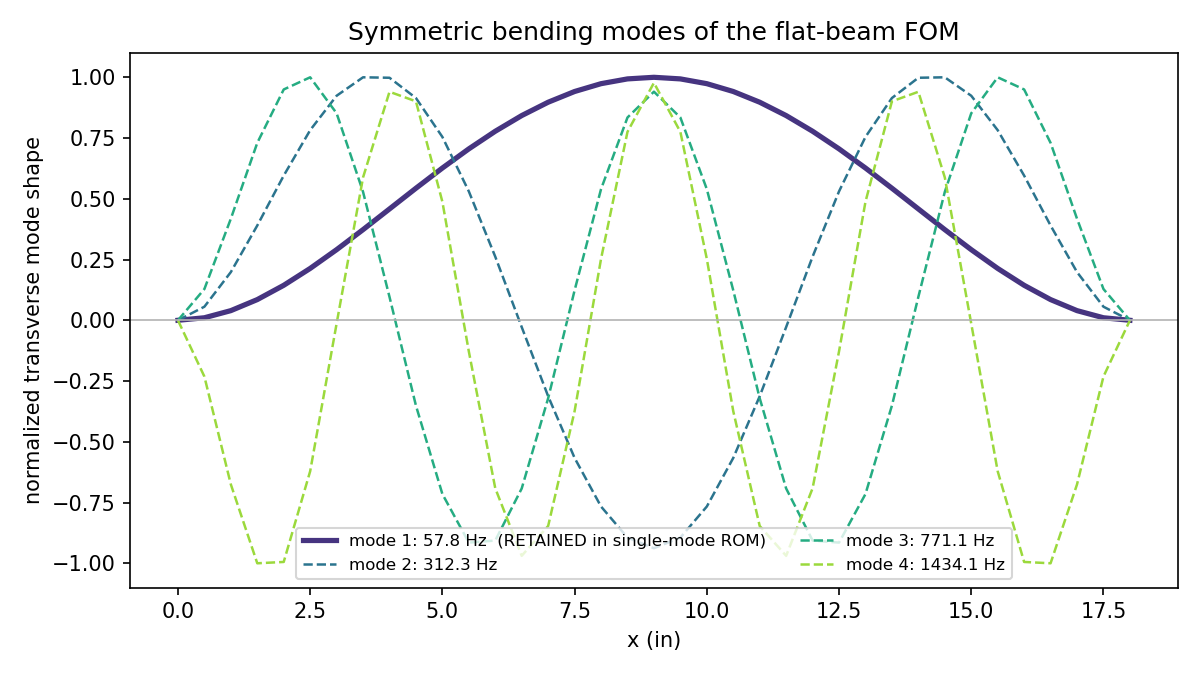
\includegraphics[width=0.85\linewidth]{figures/ch14r/ice_modes.png}
\caption{The four retained symmetric bending modes. The one-mode ROM keeps only the first. Plot of the reproduction report.}\label{fig:vf-ice-modes}
\end{figure}

\subsection*{Results: one-mode dynamics}

\Cref{fig:vf-ice} shows the displacement at $x=4$~in and its power spectral density for the two levels. At the low level the ROM follows the waveform and the first-mode peak and misses the peaks near 312 and 1400~Hz (modes not retained); at the high level it follows the full-order response for about 0.1~s and then loses phase. The errors are $19.5\,\%$ (low) and $136\,\%$ (high) for the first set of settings; the peak $|q_{\rm nl}|$ is $1.1\times10^{-4}$ at the low level and $5.8\times10^{-3}$ at the high level against a training peak of $7.4\times10^{-3}$.

\begin{figure}[tbp]
\centering
\includegraphics[width=0.9\linewidth]{figures/ch14_ice.pdf}
\caption{One-mode ICE ROM against the full-order model for the flat beam of \citet{hollkamp2008ice}: displacement at $x=4$~in over the first $0.2$~s and its power spectral density, at the low level (RMS error \cvfIceLowRms) and the high level (RMS error \cvfIceHighRms). Redrawn by \texttt{scripts/ch14\_assets.py} from the saved outputs of the study; the study itself was not re-run for this book.}\label{fig:vf-ice}
\end{figure}

\emph{Why two one-mode runs differ at the high level.} Two scripts ran the one-mode case with different ROMs against the same full-order response (the saved histories match exactly, same load seed). \Cref{tab:vf-ice-two} lists them; a study crossing the two training sets with both clamp multipliers (6 and 20 times the training peak) and three training seeds follows in \Cref{tab:vf-ice-seeds}.

\begin{table}[tbp]
\centering\footnotesize
\caption{The two one-mode ROMs.}\label{tab:vf-ice-two}
\begin{tabular}{@{}lllllrr@{}}
\toprule
Script & Training & Peak training $|q_{\rm nl}|$ & Cubic coefficient & Clamp & $\varepsilon$ low & $\varepsilon$ high\\
\midrule
\texttt{reproduce\_flat\_beam.py} & 60 samples, $\pm150$ (A) & $7.4\times10^{-3}$ & $5.45\times10^{10}$ & 6$\times$ & 0.1946 & 1.362\\
\texttt{reproduce\_fig1.py} & 20 samples, $\pm3$ (B) & $1.5\times10^{-3}$ & $6.61\times10^{10}$ & 20$\times$ & 0.1944 & 1.145\\
\bottomrule
\end{tabular}
\end{table}

\begin{table}[tbp]
\centering\footnotesize
\caption{One-mode study over training set, clamp and training seed.}\label{tab:vf-ice-seeds}
\begin{tabular}{@{}lrrl@{}}
\toprule
Training set & $\varepsilon$ low (all seeds, both clamps) & $\varepsilon$ high, seeds 0 / 1 / 2 & Range\\
\midrule
A (60 samples, $\pm150$) & 0.1946 & 1.362 / 1.261 / 1.258 & 1.26--1.36\\
B (20 samples, $\pm3$) & 0.1944 & 1.145 / 1.118 / 1.147 & 1.12--1.15\\
\bottomrule
\end{tabular}
\end{table}

The clamp has no effect (the ROM never reaches either bound, so 6 and 20 times give identical errors to every digit). The cubic coefficient differs by about $21\,\%$ between the sets, and at the high level the two ROMs reach similar peaks (about $5$--$6\times10^{-3}$) but follow different trajectories; why the wider-amplitude set fits softer was not tested, and a non-cubic component of the true force at larger amplitude is one possibility. Seed sensitivity is modest (about $0.1$ for set A, $0.03$ for set B, none at the low level; only the training seed was varied, not the load seed). The conclusion is unchanged: every one-mode ROM exceeds 1 at the high level, and the figure to quote is $1.12$--$1.36$.

\subsection*{Results: in-plane displacement}

\Cref{fig:vf-ice-inplane} compares the in-plane spectrum at $x=4$~in of the full-order model with the one-mode ICE model and membrane expansion. At the high level the spectra agree below about 400~Hz and the expanded response then falls away by many orders of magnitude; at the low level the model lacks the spectral peaks of the full-order response. With one mode \cref{eq:ice-exp} gives $u(t)=T_mp_1(t)^2$ and $p_1^2\ge0$, so the predicted in-plane motion keeps one sign and follows a slow envelope while the full-order motion oscillates about zero. This is a limit of the one-mode expansion, independent of the quality of the fit. Peak in-plane values at the high level are $3.89\times10^{-3}$~in (full order) and $2.34\times10^{-3}$~in (ROM).

\begin{figure}[tbp]
\centering
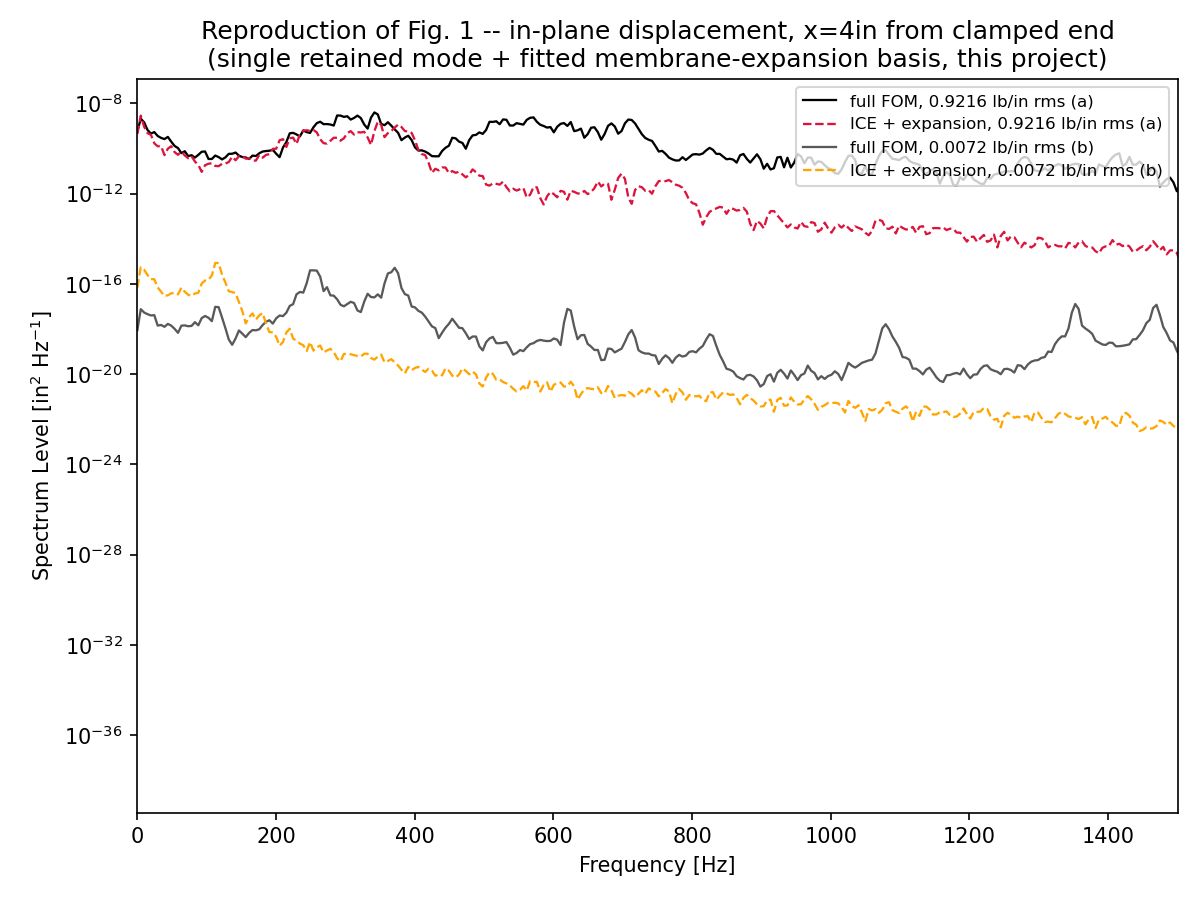
\includegraphics[width=0.8\linewidth]{figures/ch14r/ice_inplane.png}
\caption{In-plane displacement spectrum at $x=4$ in. Solid: full-order model; dashed: single-mode ICE with membrane expansion. Upper pair: high level; lower pair: low level. Plot of the reproduction report.}\label{fig:vf-ice-inplane}
\end{figure}

\subsection*{Results: four modes and the training distribution}

\Cref{tab:vf-ice-four} and \Cref{fig:vf-ice-variants} give the four-mode variants. The restricted form of \cref{eq:ice-restr} is worse than the unrestricted one in this comparison; adding states from short full-order transients (trajectory-piloted samples) improves both levels, by a factor of about $3$ at the low level and $1.5$ at the high level, and does not bring the high level below 1. A neural surrogate with static $R^2=0.99935$ diverges: the reduced response grows to a peak of about 78~in in the first 0.2~s while the full-order response peaks at $0.0045$~in (low) and $0.24$~in (high) (\Cref{fig:vf-ice-neural}).

\begin{table}[tbp]
\centering\footnotesize
\caption{Four-mode dynamics by variant.}\label{tab:vf-ice-four}
\begin{tabular}{@{}lrr@{}}
\toprule
Variant & $\varepsilon$ low & $\varepsilon$ high\\
\midrule
Polynomial, restricted form, static samples only & 0.336 & 7.93\\
Polynomial, unrestricted, static samples only & 0.0645 & 2.00\\
Polynomial, unrestricted, static + trajectory-piloted samples & 0.0219 & 1.35\\
Neural surrogate (MLP), static samples only & $3.3\times10^{4}$ & 538\\
\bottomrule
\end{tabular}
\end{table}

\begin{figure}[tbp]
\centering
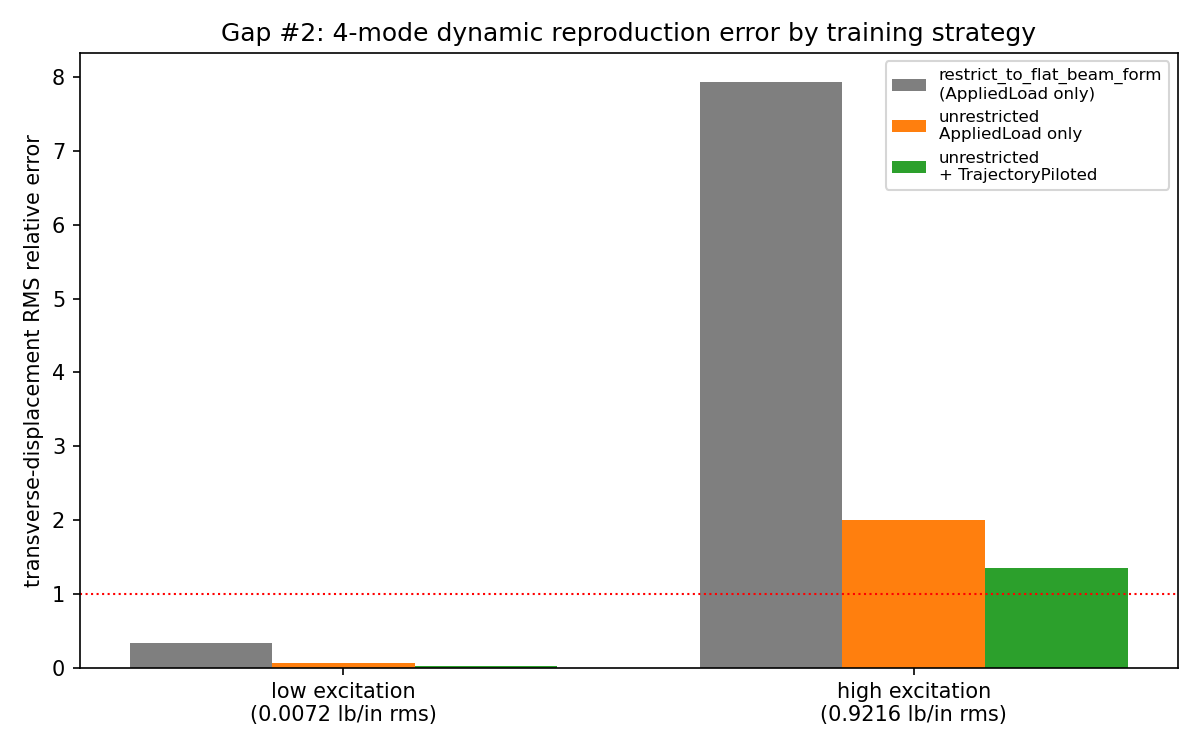
\includegraphics[width=0.7\linewidth]{figures/ch14r/ice_variants.png}
\caption{Four-mode RMS error by training strategy; the dotted line at 1 marks an error equal to the full-order signal. Plot of the reproduction report.}\label{fig:vf-ice-variants}
\end{figure}

\begin{figure}[tbp]
\centering
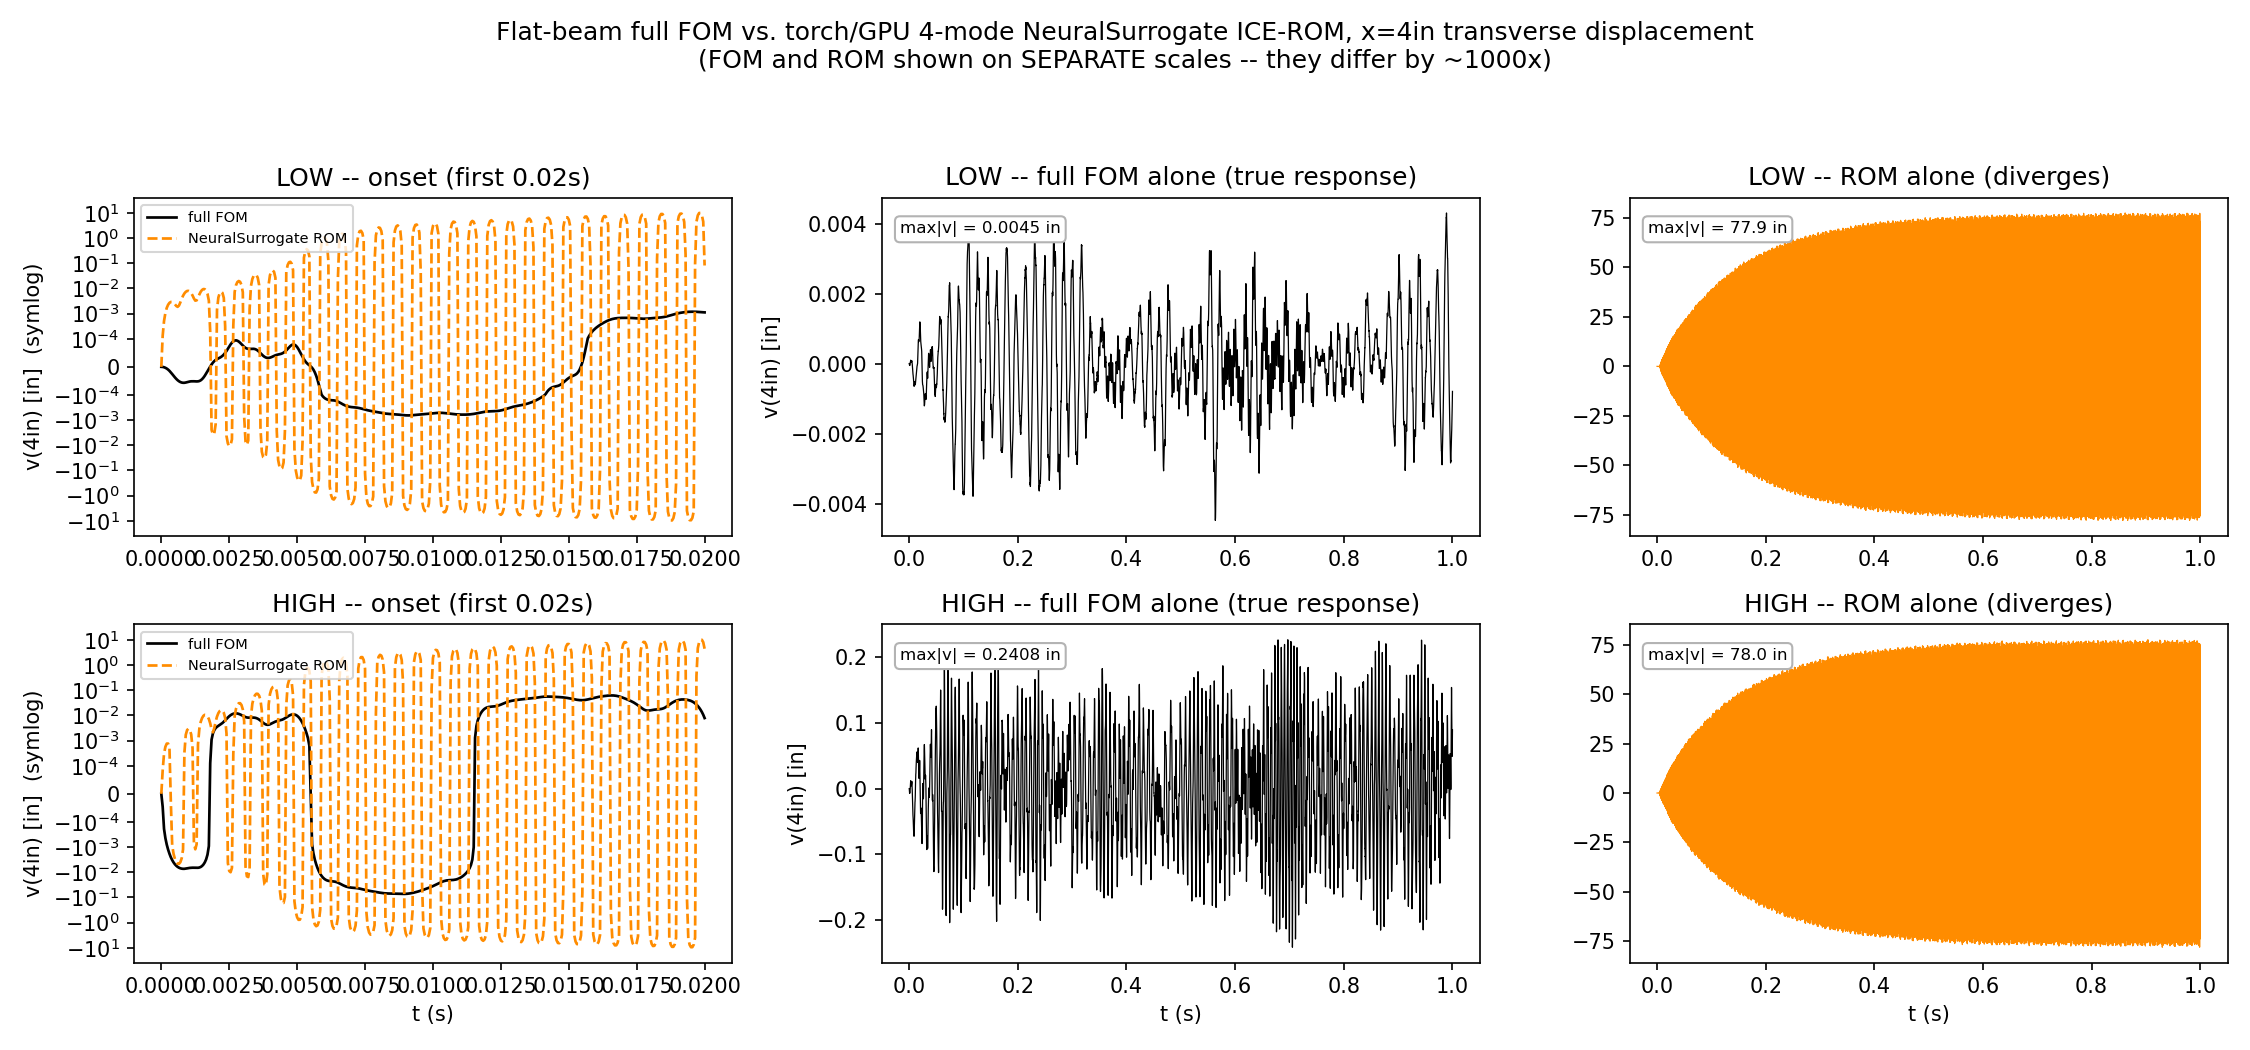
\includegraphics[width=0.8\linewidth]{figures/ch14r/ice_neural.png}
\caption{Four-mode neural ICE ROM against the full-order model, on separate scales about 1000 times apart. Plot of the reproduction report.}\label{fig:vf-ice-neural}
\end{figure}

Two regressors of different type, with static $R^2$ above $0.999$, fail in the same way, which points at the training distribution and not at the regression: the static sampling strategy draws each mode's target displacement independently, whereas a random response visits coupled, sign-varying combinations. Adding states from full-order transients reduces the four-mode error by a factor of $1.5$ to $3$, consistent with a coverage problem. Whether broader or iterated training (refit, re-simulate, add points where ROM and full-order response disagree) brings the high level below 1 was not run.

\subsection*{Results: integrator and stress recovery}

The reduced Newton--Newmark routine of the package, \texttt{integrate\_newmark\_surrogate} with \texttt{correction='newton'}, matches the study's prototype integrator exactly: over 0.1~s on the four-mode case the maximum absolute difference in $q_{\rm nl}$ is exactly 0 (\Cref{fig:vf-ice-integ}). The built-in lag-correction schemes diverged to NaN on the polynomial model, which is why the prototype was written. Stress recovery by \cref{eq:ice-stress} was evaluated for one training snapshot with 0.31~in peak transverse amplitude (\Cref{fig:vf-ice-stress}): along element~7 the mid-plane (membrane) stress is $22.4$~ksi, the top fibre about $26$--$27$~ksi and the bottom fibre about $18$--$19$~ksi, so the membrane part dominates, as the publication relies on. This was not checked against full-order element stresses and so does not validate the publication's stress-PSD figures.

\begin{figure}[tbp]
\centering
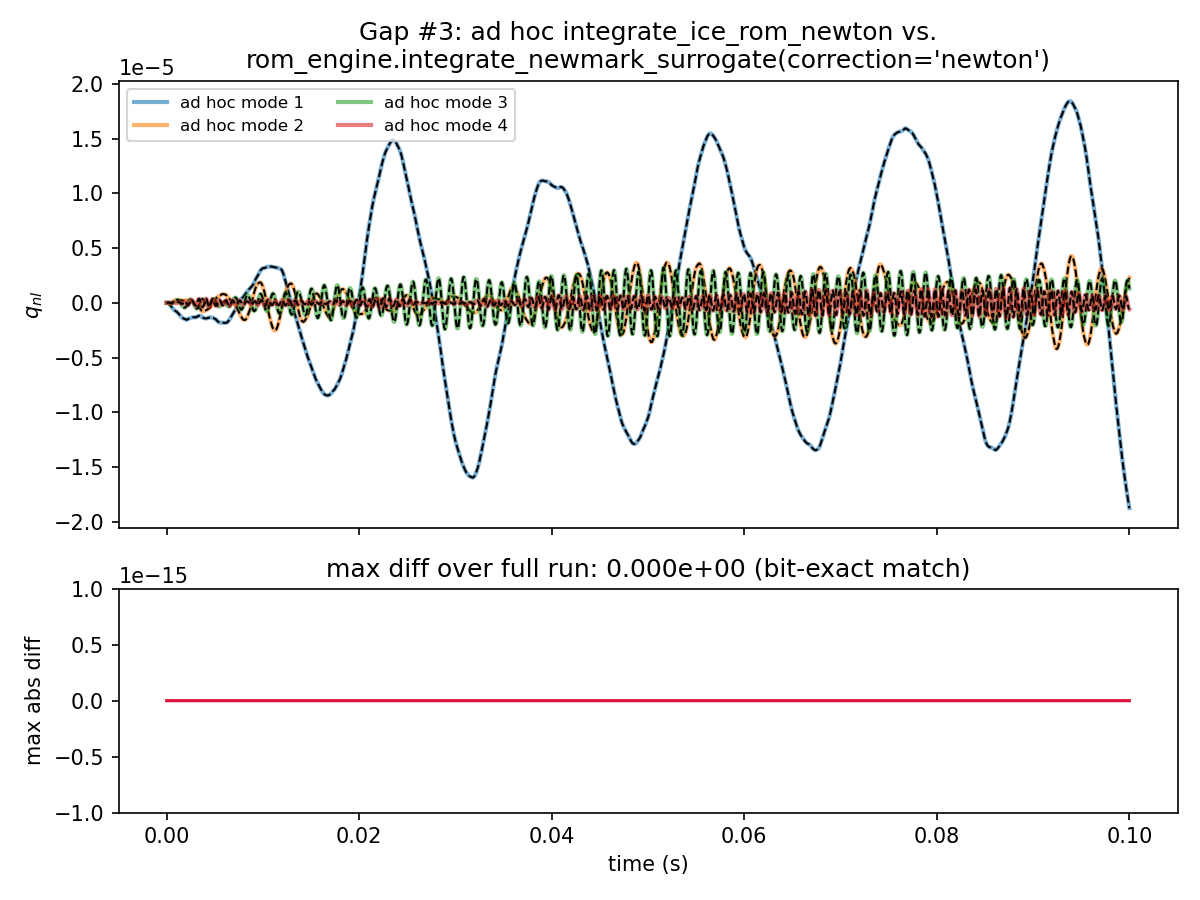
\includegraphics[width=0.8\linewidth]{figures/ch14r/ice_integrator.png}
\caption{Modal trajectories from the prototype integrator (colour) and the package routine (black dashed), with the difference below. Plot of the reproduction report.}\label{fig:vf-ice-integ}
\end{figure}

\begin{figure}[tbp]
\centering
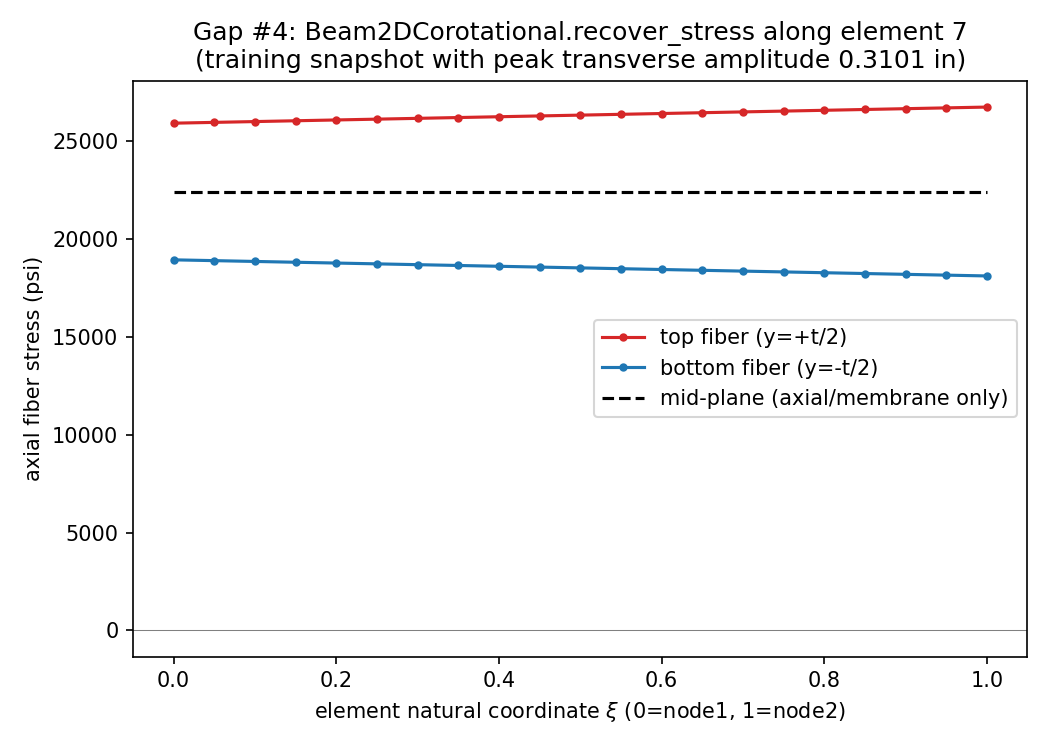
\includegraphics[width=0.7\linewidth]{figures/ch14r/ice_stress.png}
\caption{Axial stress along element 7 for a training snapshot with 0.31 in peak transverse amplitude. Plot of the reproduction report.}\label{fig:vf-ice-stress}
\end{figure}

\subsection*{Comparison with the publication}

\begin{table}[tbp]
\centering\footnotesize
\caption{Claims of \citet{hollkamp2008ice} and the outcome of the reproduction.}\label{tab:vf-ice-cmp}
\begin{tabularx}{\linewidth}{@{}>{\raggedright\arraybackslash}p{4.0cm} >{\raggedright\arraybackslash}X >{\raggedright\arraybackslash}p{2.3cm}@{}}
\toprule
Claim & This work & Outcome\\
\midrule
Linear modes (Table~2) & $57.8/312.3/771.1/1434.1$ against $57.8/312.1/770.3/1431.2$ Hz & reproduced\\
Nonlinear force identified from static solutions & held-out $R^2$ 0.9998 (1 mode), 0.99935--0.99998 (4 modes) & reproduced\\
Accurate random response, low level & $19.5\,\%$ (1 mode); $2.2$--$33.6\,\%$ (4 modes, by variant) & partly\\
Accurate random response, high level & $112$--$136\,\%$ (1 mode); $135$--$793\,\%$ (4 modes) & not reproduced\\
Membrane expansion recovers in-plane displacement (Fig.~1) & agrees below about 400 Hz at the high level only; one-sign signal & not reproduced\\
Stress recovery from the expanded field & implemented, one snapshot, no full-order comparison & not validated\\
\bottomrule
\end{tabularx}
\end{table}

\subsection*{What was not reproduced, and why}

The comparison is of the ROM against the full-order model, not an overlay of the publication's plots, so ``not reproduced'' is judged from error levels, and the publication's own dynamic accuracy figures were not extracted from the PDF. Several settings that the publication does not give (damping, time step, training sizes, the load realisation) were chosen here and can change the numbers. The one-mode case has a three-seed study on the training seed only; the four-mode variants are one training run each, and differences between them below a factor of about 2 should not be read as significant. The membrane expansion is implemented for one mode only; whether a four-mode $\mathbf T_m$ (ten quadratic terms in \cref{eq:ice-exp}) repairs the in-plane spectrum was not tried. Stress recovery has no full-order comparison. Finally, why a wider training amplitude gives a softer cubic coefficient was measured but not explained.

\Cref{tab:vf-ice-gaps} records what the study predicted from the package gap analysis and what happened.

\begin{table}[tbp]
\centering\footnotesize
\caption{Package gaps found before the study and their outcome.}\label{tab:vf-ice-gaps}
\begin{tabularx}{\linewidth}{@{}>{\raggedright\arraybackslash}p{4.2cm} >{\raggedright\arraybackslash}X@{}}
\toprule
Gap & Outcome\\
\midrule
Membrane basis and expansion missing & implemented for one mode; result above\\
Multi-mode training strategy missing & confirmed by experiment; the trajectory-piloted prototype helps by a factor $1.5$--$3$, not enough at the high level\\
Robust reduced Newton integrator missing & promoted to the package; bit-exact against the prototype\\
Fibre stress recovery missing & \texttt{Beam2DCorotational.recover\_stress} plotted for one snapshot; not validated\\
Band-limited forcing generator missing & ad hoc version used in all runs\\
\bottomrule
\end{tabularx}
\end{table}
